\documentclass[a4 paper]{article}
\usepackage[inner=2.0cm,outer=2.0cm,top=2.5cm,bottom=2.5cm]{geometry}
\usepackage{setspace}
\usepackage[rgb]{xcolor}
\usepackage{verbatim}
\usepackage{subcaption}
\usepackage{amsgen,amsmath,amstext,amsbsy,amsopn,tikz,amssymb}
\usepackage{fancyhdr}
\usepackage[colorlinks=true, urlcolor=blue,  linkcolor=blue, citecolor=blue]{hyperref}
\usepackage[colorinlistoftodos]{todonotes}
\usepackage{rotating}
\usepackage{booktabs}
\newcommand{\ra}[1]{\renewcommand{\arraystretch}{#1}}

\newtheorem{thm}{Theorem}[section]
\newtheorem{prop}[thm]{Proposition}
\newtheorem{lem}[thm]{Lemma}
\newtheorem{cor}[thm]{Corollary}
\newtheorem{defn}[thm]{Definition}
\newtheorem{rem}[thm]{Remark}
\numberwithin{equation}{section}

\newcommand{\homework}[6]{
   \pagestyle{myheadings}
   \thispagestyle{plain}
   \newpage
   \setcounter{page}{1}
   \noindent
   \begin{center}
   \framebox{
      \vbox{\vspace{2mm}
    \hbox to 6.28in { {\bf CSE 211:~Discrete Mathematics \hfill {\small (#2)}} }
       \vspace{6mm}
       \hbox to 6.28in { {\Large \hfill #1  \hfill} }
       \vspace{6mm}
       \hbox to 6.28in { {\it Instructor: {\rm #3} \hfill  {\rm #5} \hfill  {\rm #6}} \hfill}
       \hbox to 6.28in { {\it Assistant: #4  \hfill #6}}
      \vspace{2mm}}
   }
   \end{center}
   \markboth{#5 -- #1}{#5 -- #1}
   \vspace*{4mm}
}

\newcommand{\problem}[2]{~\\\fbox{\textbf{Problem #1}}\hfill (#2 points)\newline\newline}
\newcommand{\subproblem}[1]{~\newline\textbf{(#1)}}
\newcommand{\D}{\mathcal{D}}
\newcommand{\Hy}{\mathcal{H}}
\newcommand{\VS}{\textrm{VS}}
\newcommand{\solution}{~\newline\textbf{\textit{(Solution)}} }

\newcommand{\bbF}{\mathbb{F}}
\newcommand{\bbX}{\mathbb{X}}
\newcommand{\bI}{\mathbf{I}}
\newcommand{\bX}{\mathbf{X}}
\newcommand{\bY}{\mathbf{Y}}
\newcommand{\bepsilon}{\boldsymbol{\epsilon}}
\newcommand{\balpha}{\boldsymbol{\alpha}}
\newcommand{\bbeta}{\boldsymbol{\beta}}
\newcommand{\0}{\mathbf{0}}


\begin{document}
\homework{Homework \#1}{Due: 17/11/20}{Dr. Zafeirakis Zafeirakopoulos}{Gizem S\"ung\"u}{}{}
\textbf{Course Policy}: Read all the instructions below carefully before you start working on the assignment, and before you make a submission.
\begin{itemize}
\item It is not a group homework. Do not share your answers to anyone in any circumstance. Any cheating means at least -100 for both sides. 
\item Do not take any information from Internet.
\item No late homework will be accepted. 
\item For any questions about the homework, send an email to gizemsungu@gtu.edu.tr
\item The homeworks (both latex and pdf files in a zip file) will be
submitted into the course page of Moodle.
\item The latex, pdf and zip files of the homeworks should be saved as
"Name\_Surname\_StudentId".$\{$tex, pdf, zip$\}$.
\item If the answers of the homeworks have only calculations without any formula or any explanation -when needed- will get zero.
\item Writing the homeworks on Latex is strongly suggested. However, hand-written paper is still accepted $\textbf{IFF}$ hand writing of the student is clear and understandable to read, and the paper is well-organized. Otherwise, the assistant cannot grade the student's homework.
\end{itemize}

\problem{1: Conditional Statements}{5+5+5=15}
State the converse, contrapositive, and inverse of each of these conditional statements.


\subproblem{a} If it snows tonight, then I will stay at home.
\solution
%%%%%%REMOVE \newline commands while writing your answer%%%%%
\newline
\newline
\textbf{Converse:}
If I stay at home, then it will snow tonight.
\newline
\newline
\textbf{Contrapositive:}
If I don't stay at home, then it won't snow tonight.
\newline
\newline
\textbf{Inverse:}
If it doesn't snow tonight, then I won't stay at home.
\newline




\subproblem{b} I go to the beach whenever it is a sunny summer day.
\solution
%%%%%%REMOVE \newline commands while writing your answer%%%%%
\newline
\newline
\textbf{Converse:}
It is a sunny summer day whenever I go to the beach.
\newline
\newline
\textbf{Contrapositive:}
It is not a sunny summer day whenever I don't go to the beach.
\newline
\newline
\textbf{Inverse:}
I don't go to the beach whenever it is not a sunny summer day.
\newline
\newline
\newline
\newline
\newline


\subproblem{c} If I stay up late, then I sleep until
noon.
\solution
%%%%%%REMOVE \newline commands while writing your answer%%%%%
\newline
\newline
\textbf{Converse:}
If I sleep until noon, then I stay up late.
\newline
\newline
\textbf{Contrapositive:}
If I don't sleep until noon, then I don't stay up late.
\newline
\newline
\textbf{Inverse:}
If I don't stay up late, then I don't sleep until noon.
\newline
\newline


\problem{2: Truth Tables For Logic Operators}{5+5+5=15}
Construct a truth table for each of the following compound propositions.
\subproblem{a} (p $\oplus$ $\neg$ q)
\solution
%%%%%%REMOVE \newline commands while writing your answer%%%%%
\newline
\newline
$\oplus$ gives true value when either first or second condition is true but not both.
\newline
\newline
   \underline{p}  \hspace{1.2cm} \underline{$\neg$q}    \hspace{1cm}  \underline{p $\oplus$ $\neg$ q}
\newline
\newline
    T \hspace{1.2cm} T \hspace{1.5cm} F
\newline
    T \hspace{1.2cm} F \hspace{1.5cm} T
\newline
    F \hspace{1.2cm} T \hspace{1.5cm} T
\newline
    F \hspace{1.23cm} F \hspace{1.5cm} F
\newline
\newline

\subproblem{b} (p $\iff$ q) $\oplus$ ( $\neg$ p $\iff$ $\neg$ r)
\solution 
%%%%%%REMOVE \newline commands while writing your answer%%%%%
\newline
\newline
    $\iff$ gives true value only when both first and second condition is true or false. 
\newline
\newline
    \underline{p}                       \hspace{1cm} 
    \underline{$\neg$p}                 \hspace{1cm} 
    \underline{q}                       \hspace{1cm}
    \underline{$\neg$r}                 \hspace{1cm}
    \underline{p $\iff$ q}              \hspace{1cm}
    \underline{$\neg$p $\iff$ $\neg$r}  \hspace{1cm}
    \underline{(p $\iff$ q)$\oplus$($\neg$p $\iff$ $\neg$r)}
\newline
\newline
    T \hspace{1cm} F \hspace{1.1cm} T \hspace{1cm} T \hspace{1.7cm} T \hspace{2.45cm} F \hspace{3.5cm} T
\newline
    T \hspace{1cm} F \hspace{1.1cm} T \hspace{1cm} F \hspace{1.7cm} T \hspace{2.45cm} T \hspace{3.5cm} F
\newline
    T \hspace{1cm} F \hspace{1.1cm} F \hspace{1cm} T \hspace{1.7cm} F \hspace{2.45cm} F \hspace{3.5cm} F
\newline
    T \hspace{1cm} F \hspace{1.1cm} F \hspace{1cm} F \hspace{1.7cm} F \hspace{2.45cm} T \hspace{3.5cm} T
\newline
    F \hspace{1cm} T \hspace{1.1cm} T \hspace{1cm} T \hspace{1.7cm} F \hspace{2.45cm} T \hspace{3.5cm} T
\newline
    F \hspace{1cm} T \hspace{1.1cm} T \hspace{1cm} F \hspace{1.7cm} F \hspace{2.45cm} F \hspace{3.5cm} F
\newline
    F \hspace{1cm} T \hspace{1.1cm} F \hspace{1cm} T \hspace{1.7cm} T \hspace{2.45cm} T \hspace{3.5cm} F
\newline
    F \hspace{1cm} T \hspace{1.1cm} F \hspace{1cm} F \hspace{1.7cm} T \hspace{2.45cm} F \hspace{3.5cm} T
\newline

\subproblem{c} (p $\oplus$ q) $\Rightarrow$ (p $\oplus$ $\neg$ q)
\solution
\newline
\newline
    $\Rightarrow$ gives false value only when the first condition is true and second one is false.
\newline
\newline
    \underline{p} \hspace{1.1cm}
    \underline{q} \hspace{0.9cm}
    \underline{$\neg$q} \hspace{1cm}
    \underline{p $\oplus$ q} \hspace{1cm}
    \underline{p $\oplus$ $\neg$q} \hspace{1cm}
    \underline{(p $\oplus$ q) $\Rightarrow$ (p $\oplus$ $\neg$q)}
\newline
\newline
    T \hspace{1cm} T \hspace{1cm} F \hspace{1.4cm} T \hspace{1.7cm} F \hspace{2.8cm} F
\newline
    T \hspace{1cm} F \hspace{1cm} T \hspace{1.4cm} F \hspace{1.7cm} T \hspace{2.8cm} T
\newline
    F \hspace{1cm} T \hspace{1cm} F \hspace{1.4cm} F \hspace{1.7cm} T \hspace{2.8cm} T
\newline
    F \hspace{1cm} F \hspace{1cm} T \hspace{1.4cm} T \hspace{1.7cm} F \hspace{2.8cm} F
\newpage


\problem{3: Predicates and Quantifiers}{21}
There are three predicate logic statements which represent English sentences as follows.

\begin{itemize}
	\item P(x): "x can speak English."
	\item Q(x): "x knows Python."
	\item H(x): "x is happy."
\end{itemize}

Express each of the following sentences in terms of P(x), Q(x), H(x), quantifiers, and logical connectives or vice versa. The domain
for quantifiers consists of all students at the university.

\subproblem{a} There is a student at the university who can speak English and who knows Python.
\solution
\newline
\newline
    $\exists$\hspace{0.05cm}x(P(x)$\wedge$\hspace{0.05cm}Q(x))
\newline
\newline
\subproblem{b} There is a student at the university who can speak English but who doesn’t know Python.
\solution
\newline
\newline    
    $\exists$\hspace{0.05cm}x(P(x)$\wedge$\hspace{0.05cm}$\neg$Q(x))
\newline
\newline
\subproblem{c} Every student at the university either can speak English or knows Python.
\solution
\newline
\newline    
    $\forall$\hspace{0.05cm}x(P(x)$\vee$\hspace{0.05cm}Q(x))
\newline
\newline
\subproblem{d} No student at the university can speak English or knows Python.
\solution
\newline
\newline    
    $\neg$\hspace{0.05cm}$\forall$\hspace{0.05cm}x(P(x)$\vee$\hspace{0.05cm}Q(x))
\newline
\newline
\subproblem{e} If there is a student at the university who can speak English and know Python, then she/he is happy.
\solution
\newline
\newline    
    (P(x)$\wedge$\hspace{0.05cm}Q(x)) $\Rightarrow$ H(x)
\newline
\newline
\subproblem{f} At least two students are happy.
\solution
\newline
\newline    
    $\exists$\hspace{0.05cm}$x_1$\hspace{0.05cm}$\exists$\hspace{0.05cm}$x_2$
    (H($x_1$) $\wedge$ H($x_2$) $\wedge$ ($x_1$ $\neq$ $x_2$)) 
\newline    
\newline
    (** Without ($x_1$ $\neq$ $x_2$) it means there are at least one happy student. By providing ($x_1$ $\neq$ $x_2$) we make sure that we have at least two different students who are happy. **)
\newline
\newline
\subproblem{g} $\neg \forall x (Q(x) \wedge P(x))$
\solution
%%%%%%REMOVE \newline commands while writing your answer%%%%%
\newline
\newline
    No student at the university knows Python and can speak English.
\newline
\newline
\newline
\problem{4: Mathematical Induction}{21}
Prove that 3 + 3 . 5 + 3 . $5^2$ + . . . + 3 . $5^n$ =$\frac{3(5^{n+1} - 1)}{4}$
whenever n is a nonnegative integer.
\solution
\newline
\newline
** First we do basis step to show our equation is true. ** 
\newline
\newline
%%%%%%REMOVE \newline commands while writing your answer%%%%%
(For n = 0) $ \rightarrow 3.5^{0} = \dfrac{3.(5^{0+1}-1)}{4} 
              \rightarrow 3.1 = \dfrac{3.(5 - 1)}{4} 
              \rightarrow 3 = \dfrac{12}{4} 
              \rightarrow 3 = 3 $ (basis step is correct)
\newline
\newline
** Second we start our inductive step. We assume that n = k satisfies the equation.
\newline
\newline
(For n = k) $\rightarrow \hspace{0.2cm} 3.5^{0} + 3.5^{1} + ... + 3.5^{k} = \dfrac{3.(5^{k+1}-1)}{4}$
\newline
\newline
** Then finally we put the equation from where we assumed that n = k satisfied the function to n = k + 1. If the equation turns out to be true then that means we proved our equation. ** 
\newline
\newline
(For n = k+1) $\rightarrow \hspace{0.2cm} 3.5^{0} + 3.5^{1} + ... + 3.5^{k} + 3.5^{(k+1)} = \dfrac{3.(5^{(k+1)+1}-1)}{4}
               \rightarrow \hspace{0.2cm} \dfrac{3.(5^{k+1}-1)}{4} + 3.5^{(k+1)}  = \dfrac{3.(5^{k+2}-1)}{4}
\newline\newline
\hspace{0.2cm} \rightarrow \hspace{0.2cm} 5^{(k+1)} = \dfrac{(5^{k+2}-1) - (5^{k+1}-1)}{4}
                                                    = \dfrac{5^{k+2} - 5^{k+1}}{4}
                                                    = \dfrac{5^{k+1}.(5-1)}{4} = 5^{(k+1)}
              $ 
\newline
\newline
\problem{5: Mathematical Induction}{20}
Prove that $n^2$ - 1 is divisible by 8 whenever n is an odd
positive integer.
\solution
%%%%%%REMOVE \newline commands while writing your answer%%%%%
\newline
\newline
** Again first we do our basis step to show our equation is true. **
\newline
\newline
(For n = 3)    $  \rightarrow \hspace{0.2cm} \dfrac{3^2-1}{8} = 1  $
\newline
\newline
** Now we rebuild the equation for n = 2k+1. (k $\in\mathbb{N}$) ** 
\newline
\newline
(For n = 2k+1) $  \rightarrow \hspace{0.2cm} (2k+1)^2-1  $
               $ =\hspace{0.1cm} (4k^2+4k+1)-1           $
               $ =\hspace{0.1cm} 4k^2+4k                 $
               $ =\hspace{0.1cm} 4k(k+1)                 $
\newline
\newline
** Finally we assume that 4k(k+1) is dividable by 8. We try to find this pattern with n = 2(k+1)+1. If we can that means n2- 1 is dividable by 8 whenever n is an odd positive integer.** 
\newline
\newline
(For n = 2(k+1)+1) $  \rightarrow \hspace{0.1cm} (2(k+1)+1)^2-1  $
                   $ =\hspace{0.1cm} (2k+3)^2-1        $
                   $ =\hspace{0.1cm} 4k^2 + 12k + 8    $
                   $ =\hspace{0.1cm} 4(k^2 + 3k + 2)   $
                   $ =\hspace{0.1cm} 4(k+1)(k+2)       $
\newline          
** 4 * (k+1) divides 8 since k+1 is dividable by 2. **                 
\newline               
\newline
\problem{6: Sets}{8}
Which of the following sets are equal? Show your work step by step.\newline
\subproblem{a} $\{$t : t is a root of $x^2$ – 6x + 8 = 0$\}$
\newline
\subproblem{b} $\{$y : y is a real number in the closed interval [2, 3]$\}$
\newline
\subproblem{c} $\{$4, 2, 5, 4$\}$
\newline
\subproblem{d} $\{$4, 5, 7, 2$\}$ - $\{$5, 7$\}$
\newline
\subproblem{e} $\{$q: q is either the number of sides of a rectangle or the number of digits in any integer between 11 and 99$\}$\\
\solution
\newline
\newline
(a) $ t^2 - 6t + 8 = 0 \rightarrow (t-2)(t-4) = 0 \rightarrow t = 2, t = 4 $
\newline
\newline
    $ \rightarrow $ a = \{2, 4\} 
\newline
\newline
(b) since y is between closed interval we can include both 2,3 as an element of set b. so set b becomes:
\newline
\newline
    $ \rightarrow $ b = \{2, 3\} 
\newline
\newline    
(c) elements of set c is already given as (of course after we remove same elements):
\newline
\newline
    $ \rightarrow $ c = \{2, 4, 5\}
\newline
\newline    
(d) After we remove \{5,7\} elements from the given set our d set becomes:
\newline
\newline
    $ \rightarrow $ d = \{2, 4\}     
\newline
\newline    
(e) first element of set e is \{4\} since rectangles have 4 sides. And second element is \{2\} since every the integer between 11-99 has 2 digits. so set e is: 
\newline
\newline
    $ \rightarrow $ e = \{2, 4\} 
\newline
\newline
To be able to say two sets are equal their both element numbers and values must be the same. 
\newline
Equal sets are $\rightarrow$ a, d and e
\newline
\newline
\problem{Bonus: Logic in Algorithms}{20}

Let p and q be the statements as follows.

\begin{itemize}
	\item $\textbf{p:}$ It is sunny.
	\item $\textbf{q:}$ The flowers are blooming.
\end{itemize}

\begin{figure*}[htp]
	\centering
	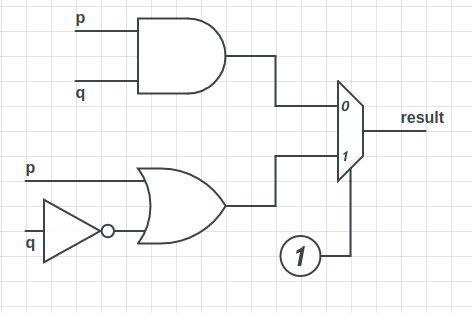
\includegraphics[scale=0.5]{circuit.png}
	\caption{Combinational Circuit}
	\label{fig: circuit}
	
\end{figure*}

In Figure \ref{fig: circuit}, the two statements are used as input. The circuit has 3 gates as AND, OR and NOT operators. It has also a 2x1 multiplexer\footnote{https://www.geeksforgeeks.org/multiplexers-in-digital-logic/} which provides to select one of the two options.
\newpage
\subproblem{a} Write the sentence that "result" output has.
\solution 
\newline
\newline
    Since multiplexer shows 1, we won't consider 0 as a part of the circuit. And if we take bottom part, condition becomes to ($p\vee\neg q$) and the sentence is:
\newline
\newline
    $\rightarrow\hspace{0.2cm}$ It is sunny or the flowers are not blooming.
\newline
\subproblem{b} Convert Figure \ref{fig: circuit} to an algorithm which you can write in any programming language that you prefer (including pseudocode).
\solution 
\newline
\newline
If multipleexer is showing 1 then it will go to orOP which takes p $ and\hspace{0.1cm}\neg $q as parameters. Then returns new string with or.
\newline
For this code the output is "it is sunny or the flowers are not blooming". 
\newline
\begin{tabular}{|p{10cm}|}
  \begin{verbatim}
#include <iostream>
using namespace std;

string orOP(string p, string q)
{
    return p + " or " + q;
}

string andOP(string p, string q)
{
    return p + " and " + q;
}

int main()
{
    string p     = "it is sunny";
    string notp  = "it is not sunny";
    string q     = "the flowers are blooming";
    string notq  = "the flowers are not blooming";

    bool multiplexer = 1;

    if(multiplexer == 0)
        cout << andOP(p, q);
    else if(multiplexer == 1)
        cout << orOP(p, notq);

    return 0;
}
  \end{verbatim}
\end{tabular}
\newline
\end{document} 
